\chapter{Array} 
Um array \'e uma vari\'avel n\~ao escalar, isto \'e, possui espa\c{c}o em mem\'oria capaz de armazenar mais de um dado. Um array pode ser criado
para qualquer tipo de dado, podendo ser usado simultaneamente para diversos dados, sendo desta forma extremamente \'util, segue um exemplo na figura 25.  

\begin{figure}[!htb]
	\centering
	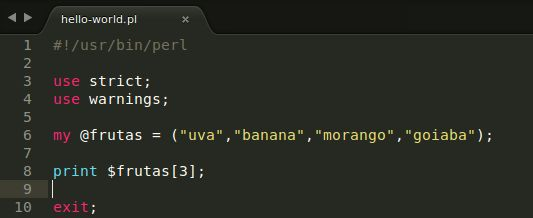
\includegraphics[width=0.4\textwidth]{../5_figuras/image25}
	\caption{Algoritmo fazendo uso de arrays}
\end{figure}

Sua sa\'ida \'e apresentada na figura 26.

\begin{figure}[!htb]
	\centering
	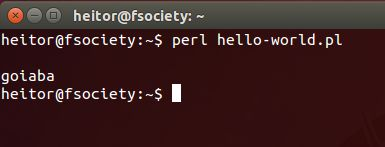
\includegraphics[width=0.3\textwidth]{../5_figuras/image26}
	\caption{Sa\'ida do algoritmo fazendo uso de arrays}
\end{figure}

Na figura 26, linha 6 \'e declarado o array da seguinte maneira usando a express\~ao \textit{my @frutas = (''uva'', ''banana'', ''morango'', ''goiaba'');}. 
Em seguida, \'e usado \textit{print} para escrever na tela o item 3, goiaba. Um array tem seu espa\c{c}o em mem\'oria contado em blocos na forma 
\textit{n-1, onde n \geqslant 1}, desta forma, se n=4 \Rightarrow, ent\~ao o espa\c{c}o dispon\'ivel para uso seria {0, 1, 2, 3}.

Para iterar sobre todas as posi\c{c}\~oes de um array \'e poss\'ivel usar-se as estruturas de repeti\c{c}\~ao apresentadas no cap\'itulo 9 al\'em do la\c{c}o
de repeti\c{c}\~ao \textit{foreach}. O \textit{foreach} consiste de um comando que \'e respons\'avel por percorrer um array de maneira simplificada, o que 
facilita acessar todas as posi\c{c}\~oes de um array, como apresentado no exemplo da figura 27.

\begin{figure}[!htb]
	\centering
	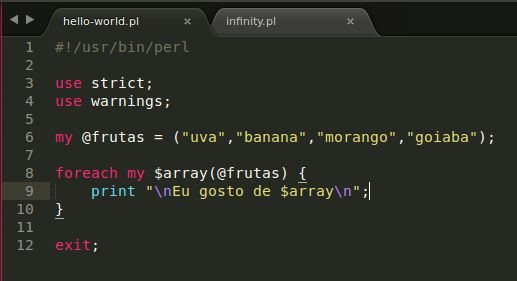
\includegraphics[width=0.6\textwidth]{../5_figuras/image27}
	\caption{Algoritmo iterando o array via foreach}
\end{figure}

Sua sa\'ida \'e apresentada na figura 28.


\begin{figure}[!htb]
	\centering
	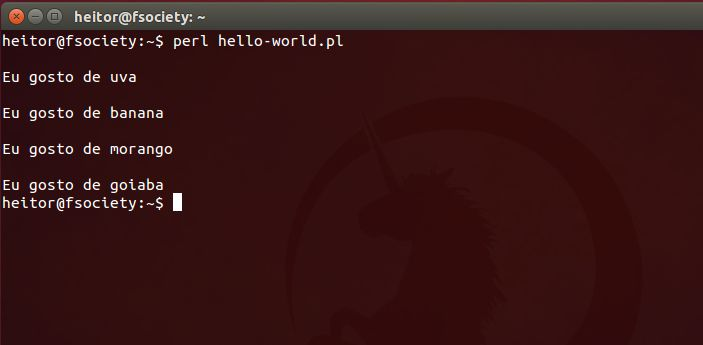
\includegraphics[width=0.3\textwidth]{../5_figuras/image28}
	\caption{Sa\'ida do algoritmo iterando o array via foreach}
\end{figure}
